\documentclass[11pt,letterpaper,twocolumn]{article}
\usepackage[utf8]{inputenc}
\usepackage[spanish]{babel}
\usepackage{amsmath}
\usepackage{amsfonts}
\usepackage{amssymb}
\usepackage{graphicx}
\usepackage{listings}
%\usepackage{fourier}
\usepackage[left=2cm,right=2cm,top=2cm,bottom=2cm]{geometry}
%\author{miguel}
\begin{document}
%Simulación en Python de un tiro parabolico bidimensional que experimenta fricción viscosa, utilizando el método de Runge Kutta.\\
\title{\huge{\textbf{
Python simulation of a two-dimensional parabolic shot experiencing viscous friction, using the Runge Kutta method.}}}
\author{\small \textit{M. Sabogal $^{1}$, H. Torres $^{1}$, M. Bandera $^{1}$, J. Gallardo $^{1}$}\\
	\small \textit{ $^{1}$ Estudiante del programa de Física, Universidad del Atlántico, Barranquilla-Colombia}}
\date{} 

\twocolumn[
\begin{@twocolumnfalse}
\maketitle
\begin{center}
{\rule[0mm]{160mm}{0.2mm}}
\end{center}
\begin{abstract}
\textit{Se simuló el lanzamiento  de una partícula de masa $m$ en dos dimensiones en un medio con una fricción turbulenta descrita por $\beta$, que varía de manera aleatoria en un pequeño intervalo, de $\beta_{min}$ hasta $\beta_{max}$; utilizando el lenguaje computacional de phyton y el runge kutta de orden 4, se generó una función que describiera la trayectoria de la partícula a partir de las condiciones iniciales $(\vec{r_{o}}, \vec{v_{o}})$. Luego se encontró la distribución de alcance máximos para $N$ lanzamientos con un ángulo $\theta$ constante. Posteriormente se encontró el ángulo y la distancia máxima en el que se optimiza el impacto de un objeto a gran distancia.\\
\\
\textbf{Palabras claves: trayectoria,fricción turbulenta, Runge Kutta.}}
\begin{center}
\textbf{Abstract} 
\end{center}
\par 
\textit{it was simulated the launching of a particle of mass $m$ in two dimensions in a medium with a turbulent friction described by $\beta$, which varies randomly in a small interval, from $\beta_{min}$ to  $\beta_{max}$; using the computational language of phyton and the runge kutta of order 4, a function that describing the trajectory of the particle was generated from the initial conditions $(\vec{r_{o}}, \vec{v_{o}})$. Then it was found the maximum range distribution for $N$ releases with a constant angle $\theta$. Subsequently, it was found the angle and the maximum distance in which the impact of an object at a great distance it is optimized.\\
\\
\textbf{Keywords: trayectory, turbuent friction, Runge Kutta.}}
\end{abstract}
\begin{center}
{\rule[0mm]{160mm}{0.2mm}}
\end{center}
\end{@twocolumnfalse}
]

\section*{\normalsize{INTRODUCCIÓN}} 
Si no hubiera gravedad se podría lanzar una pelota hacia el cielo, y esta seguiría una trayectoria recta. Sin embargo, debido a la gravedad la trayectoria que describe es una curva. Cualquiera ha golpeado una pelota de fútbol y ha intentado pasarla de su campo hasta el campo del contrario; ha lanzado una piedra, o ha visto dispar una bala. Cualquier objeto que se lanza por cualquier método, y continúa moviéndose por su propia inercia se llama proyectil; la trayectoria que el proyectil describe es una curva. En la antigüedad las trayectorias curvas de los proyectiles era algo complicado de analizar para los artilleros de guerra, hoy en día con muchas simplificaciones el problema de estas trayectorias se vuelve sorprendentemente sencillo, cuando se examinan por separado el movimiento a través de las componentes horizontales  y verticales de la velocidad.\\
\par
Si intentáramos estudiar las diferentes trayectorias curvas que observamos en el mundo real y en nuestro día a día, estas se convertirían en un problema más complicado de analizar de forma analítica, ya que influyen factores como la fricción del aire, la forma del objeto arrojado, entre otros factores involucrados en dicho movimiento. Hoy en día este problema es abordado por la “Nasa” y por otras entidades que realizan lanzamientos de satélite.
\par 
Se desea estudiar el lanzamiento de un proyectil en dos dimensiones, que se verá afectado debido a la interacción con el aire, tambien se pretende encontrar el ángulo de mayor alcance y el que de la mayor probabilidad de impacto a un objeto ubicado a una distancia “x” con respecto al origen del lanzamiento. 
\subsection*{Tiro parabólico }
Para simplificar el análisis de este tipo de movimientos, éste se considera bidimensional siempre que sea posible. En éste un cuerpo es lanzado a través de un medio o fluido (cómo el aire) por cualquier método, la trayectoria que sigue el objeto por simplicidad es una parábola, a este tipo de trayectorias se le suele llamar lanzamiento de proyectiles; en realidad, cuando se habla de cuerpos que se mueven en un campo gravitatorio central (como el de la Tierra), el movimiento es elíptico. En la superficie de la Tierra, ese movimiento es tan parecido a una parábola que perfectamente podemos calcular su trayectoria usando la ecuación matemática de una parábola, donde $\vec{r}$ es el vector posición, $\vec{v_{o}}$ el vector velocidad inicial y $\vec{a}$ el vector aceleración.

\begin{equation}
\vec{r}= \vec{r_{o}} -  \vec{v_{o}} t - \frac{1}{2} \vec{a} t^{2}
\end{equation}


\par
En un modelo realista de lanzamiento de proyectile, se debe tener en cuenta las interacciones del objeto con el fluido circundante a su alrededor. Existe un coeficiente que es utilizado en mecánica de fluidos para cuantificar si un  objeto tendrá mayor o menor resistencia en un medio o fluido como por ejemplo el agua o el aire, este depende de la forma del objeto, es decir su aerodinámica, y es proporcional a la velocidad del proyectil, además puede que surjan durante la trayectoria pequeños cambios en el fluido por el cual el objeto se está moviendo, ocasionado que sea aún más complicado la descripción de su movimiento.

\subsection*{Modelo de vuelo}
Cómo primer modelo de estudio se considera el lanzamiento de un proyectil que se mueve en un medio (aire) que presenta fricción viscosa, donde ésta fuerza viene dada por la expresión:\\
\begin{equation}
\vec{F}_{fv}= -\lambda \vec{v} - \beta v \vec{v}
\label{viscosa}
\end{equation}
\par 
Donde $\lambda$ suministra la información de la fricción no turbulenta del aire, y $\beta$ suministra la información turbulenta. En éste modelo se supondrá que el termino turbulento puede ser descrito como una perturbación aleatoria en el medio, de manera que la función analítica $\beta(t)$ es desconocida pero toma valores en un pequeño intervalo cerrado $[\beta_{min},\beta_{max}]$, y su evolución es tan rápida que puede ser descrita como una variable aleatoria distribuida uniformemente.\\
\par
A partir de la segunda ley de newton y considerando que el proyectil se mueve bajo el campo gravitatorio de la tierra, se deduce una expresión para describir la aceleración del objeto durante su trayectoria, en este caso la aceleración no depende explícitamente del tiempo, si no de la velocidad, y de los parámetros $\lambda$ y $\beta$.

\begin{equation}
\dfrac{d^{2}\vec{r}}{dt^{2}}=\vec{g}- \frac{1}{m}(\lambda \vec{v} - \beta v \vec{v})
\label{aceleracion}
\end{equation}
\par 
Donde $v$ es la magnitud del vector velocidad. La ecuación \ref{aceleracion} es una EDO de segundo orden que se debe resolver para tener pleno entendimiento del fenómeno, teniendo en consideración que $\beta$ cambia de manera aleatoria; por tanto el sistema no es enteramente determinista.   
\subsection*{Modelo de impacto}
Cómo modelo final, se considera el lanzamiento de un proyectil descrito por el modelo anterior, que es dirigido hacia un objetivo perfectamente cuadrado de lados \emph{l}, a una distancia horizontal $d$ del punto de lanzamiento.  

\section*{-Interpretación física y resultados}
Con el fin de estudiar el movimiento de un proyectil en dos dimensiones en un medio con fricción, se simulo el \textbf{modelo de vuelo}, utilizando el lenguaje de programación de python. En primera instancia se establece la localización del observador, colocando la referencia espacial $(0,0)$ en el punto del lanzamiento y el tiempo cero justo al inicio de éste. Se considera que las dimensiones del proyectil son mucho más pequeñas que las del objetivo de impacto, por la tanto se estudiará el problema tomando el proyectil como una partícula, donde la aceleración que la particula experimenta esta descrita por \ref{aceleracion}. Este modelo se estudiará desde la perspectiva de los sistemas dinámicos, permitiendo describir la evolución del sistema a partir de la evolución de la velocidad y posición en función del tiempo, es decir encontrar un vector “Y” que contenga estas cantidades. Para lograr esto se sabe que la velocidad es la derivada de la posición con respecto al tiempo y la aceleración es la derivada de la velocidad con respecto al tiempo, tomando el conjunto de estas cantidades como la derivada en el tiempo del vector dinámico $Y$, se tiene:\\ 

$$ F(Y,t)=\dfrac{dY}{dt}=(\vec{v},\vec{a})=( \dfrac{dx}{dt},\dfrac{dy}{dt},\dfrac{dv_{x}}{dt},\dfrac{dv_{y}}{dt}) $$
\par 
Al integrar esta expresión con respecto al tiempo, se obtiene la manera de cómo evoluciona el sistema.\\

$$ Y_{n}= Y_{n-1} + \int_{t_{n-1}}^{t_{n}} F(Y,t)dt  $$

\par 
A través del runge kutta de orden 4 con paso estándar de $h=10^{-2}$, se calculó el vector dinámico para el lanzamiento del proyectil transcurrido un cierto tiempo hasta que golpeara el suelo o al objetivo, partiendo de unas condiciones iniciales dadas $(\vec{r_{o}},\vec{v_{o}})$; las cuales se establecieron de manera que el proyectil partiera desde el origen, y el vector velocidad inicial estuviera descrito por $\overrightarrow{v_{o}}=(v_{o}\cos\theta,v_{o}\sin\theta)$ , donde $v_{o}$ dependerá del momentum impregnado por el lanzador y $\theta$ el ángulo de tiro.\\
\par 
El movimiento del proyectil no solo depende de las condiciones iniciales, sino de su interacción con el medio, a partir de ésta idea se estableció un set de parámetros en los cuales se define la masa del proyectil, un coeficiente fricción $\lambda$ que nos suministra la información de un medio no turbulento, y $\beta$ que varía de manera aleatoria en un pequeño intervalo, de $\beta_{min}$ hasta $\beta_{max}$ que nos dará la información de un medio turbulento.\\
\par 
Se realizó un vector de condiciones iniciales de cuatro componentes que consta de las posiciones y velocidades iniciales, desde el cual parte la integración del runge kutta, generando una matriz que representa el vector dinámico de la partícula, desde que es lanzada hasta que choca con el suelo, considerando éste cómo plano. Esto se codicionó en el rugen kutta de modo que se detuviera la integración cuando la posición en el eje $y$ de la partícula fuera menor que cero ($y<0$). Debido a el paso del runge kuta y al condicional impuesto, la última posición de la partícula se encuentra por debajo del eje $y$, es decir del suelo. Para corregrir este error se implementó una metodo de interpolación encontrando la ecuación de la recta entre los dos ultimos puntos (uno antes de $y=0$ y otro por debajo), de la cual se extrae el valor de $x$ cuando $y=0$ (ver en anexos), es decir cuando golpea el suelo.\\
\par
Se creó una clase llamada “Partícula” que contuviera la información de la trayectoria y velocidades de la partícula luego de un lanzamiento, y que tuviera un método que entregara la información estadística para un solo lanzamiento obteniendo como información la altura máxima, el tiempo que le toma en alcanzar el punto de mayor altura, y el alcance máximo con su respectivo tiempo de vuelo, a partir de un set de parámetros pre-establecidos. En la figura \ref{tra} se graficó la trayectoria de una partícula de masa $m=1$ después de un lanzamiento con velocidad inicial $v_{o}=12$, con un ángulo de tiro de $\theta=\pi/4$, con $\lambda=0.9$ y el factor de turbulencia $\beta$ en una rango entre $\beta_{min}=0$ y $\beta_{max}=0.05$ , donde se observa que la trayectoria que describe su movimiento ya no es simétrica (cómo en un tiro parabólico sin fricción) y el tiempo que tarda en alcanzar su altura máxima no es igual al tiempo de caída.    
%poner en la grafica infomacion estadistica
\begin{figure}[h!]
\centering
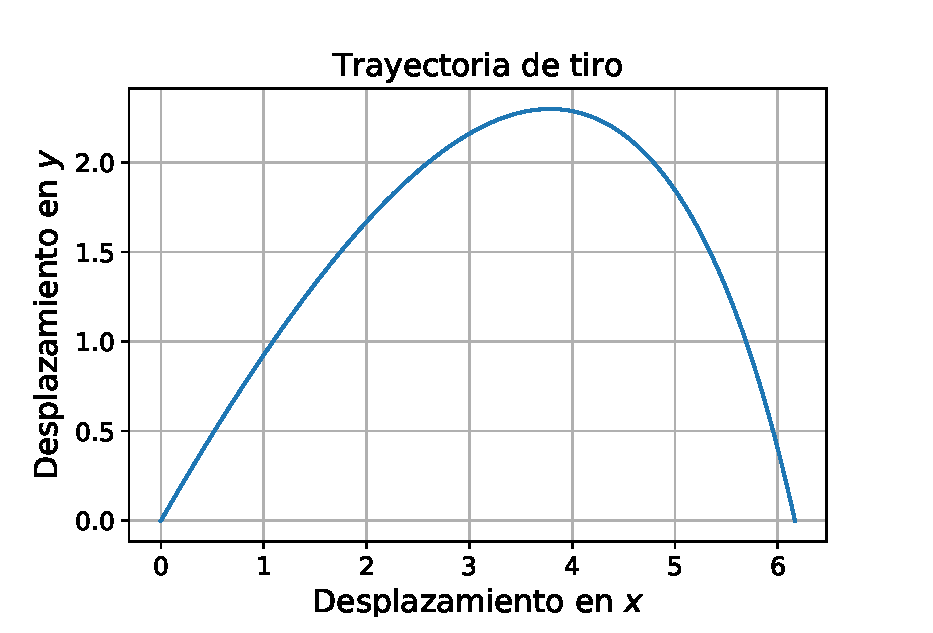
\includegraphics[scale=0.6]{tra.eps}
\label{tra}
\caption{Gráfica de la trayectoria con parámetros=[m: 1, $\lambda$: 0.9, $\beta_{min}$: 0, $\beta_{max}$: 0.05, $v_{o}$: 12, $\theta$: $\pi /4$], $h_{max}$=2.298, $x_{max}$=6.166, $time_{up}$=0.61 y $time_{fly}$=1.39.}
\end{figure}
\newpage
\par 
Con el motivo de estudiar a profundidad éste problema, que no es totalmente determinista, debido a que se cuenta con un parámetro $\beta$ que varía de forma aleatoria; se implementó una función que genere $N$ tiros con los parámetros establecidos inicialmente, y almacene la información estadística de cada uno de los lanzamientos de la muestra, y analice los resultados obtenidos de los $N$ tiros realizados por la función, con el fin de hallar los promedios y desviaciones estándar de la información estadística (altura máxima, distancia máxima y sus respectivos tiempos), paralelamente se generó un histograma de las distancias máximas obtenidas en cada tiro; tomando los puntos medios de los intervalos cómo la variable independiente, la altura de cada bin (barra) del histograma cómo la variable dependiente, y utilizando la función optimize.curve-fit de la librería Scipy se realizó el fitting del histograma, encontrando que presenta un comportamiento gaussiano, cómo se observa en la figura \ref{fiteo}, con un valor promedio de $\overline{x}_{max}=6.087$ y una desviación estándar de $\sigma=$0.0515, la cual representa la distribución del alcance máximo para $N=10.000$ lanzamientos con los mismos parámetros del lanzamiento en la figura 1. 

\begin{figure}[h!]
\centering
\includegraphics[scale=0.6]{Distribucion.eps}
\label{fiteo}
\caption{Distribución de alcance máximo, con parámetros=[m: 1, $\lambda$: 0.9, $\beta_{min}$: 0, $\beta_{max}$: 0.05, $v_{o}$: 12, $\theta$: $\pi /4$], $N=10.000$, $\overline{x}=$6.086 y $\sigma=$0.0514 }
\end{figure}

\par 
De manera subsiguiente, se definió una función donde se lanza $N$ veces un proyectil para cada ángulo, barriendo ángulos de $0$ a $90$ grados de uno en uno. Para cada grupo de $N$ lanzamientos por ángulo, sé promedio los alcances máximos, y de estos datos sé graficó en la figura \ref{alcance} el alcance máximo en función del ángulo de tiro $\theta $, donde se observa claramente la dependencia del alcance respecto al ángulo de tiro, encontrando que el ángulo que genera el alcance máximo es de $34$ grados.\\

\begin{figure}[h!]
\centering
\includegraphics[scale=0.6]{theta.eps}
\caption{Dependencia del alcance máximo en función del ángulo de tiro, con parámetros=[m: 1, $\lambda$: 0.9, $\beta_{min}$: 0, $\beta_{max}$: 0.01, $v_{o}$: 12] y $N=1$.$000$}
\label{alcance}
\end{figure}

\par 
A partir del estudio del modelo de vuelo, se procedió a introducir el objetivo del \textbf{modelo de impacto} dentro de la simulación, de manera que la integración hecha por el runge kutta se detuviera cuando golpeara el suelo o cuando la posición en el eje $y$ fuera menor o igual a \emph{l} ($y \leq \emph{l}$), y la posición en el eje $x$ estuviera entre $d$ y $d + \emph{l}$   ($d \leq x \leq d + \emph{l}$), es decir, que la partícula se encuentre dentro de las dimensiones o fronteras del objetivo. Mediante la implementación de éste modelo, se encontró que debido al tamaño del paso del runge kutta, en alguna ocasiones la partícula podría pasar por la esquina superior derecha del objetivo (según el observador) sin ser detectada, para evitar esto, se colocó una región de análisis alrededor del objetivo con la intención de realizar una interpolación entre los puntos dentro de esta región, y verificar si alguna de estas rectas cortan a $y=\emph{l}$, y si en el punto que la corta, la componente en $x$ se encuentra en el intervalo $d \leq x \leq d+ \emph{l}$, se registra que hubo un impacto en el lado superior del objetivo.\\ 

\par 
Posteriormente al modelamiento entre el choque del proyectil y el objetivo, se creó una función que lazara el proyectil con el mismo set de parámetros $N$ veces, barriendo ángulos entre 15 y 60 grados, con el objetivo a una distancia $d$ fija, y determinara la probabilidad de impacto para cada ángulo de tiro, encontrando así el ángulo que maximiza la probabilidad de impacto, para esa set de parámetros. Solo se barrieron los ángulos entre 15  y 60 grados, debido a que el alcance máximo de los ángulos $\theta < 15$ y $\theta > 60$ se encuentran muy cercanos al punto de lanzamiento, por lo tanto representan lanzamientos poco efectivos a la hora de impactar un objetivo a grandes distancias. Para una partícula de masa $m=1$ con velocidad inicial $v_{o}=12$, con $\lambda=0.9$ y el factor de turbulencia $\beta$ en una rango de $[0,0$.$05]$, se determinó que el ángulo de tiro que maximiza la probabilidad de impacto sobre el objetivo de lados $\emph{l}=0$.$1$, a una distancia $5$.$8$, es de $23$ grados con una probabilidad de impacto del $96.2\%$.\\
\par 
Análogamente se diseñó  una función que realizara el mismo barrido de la función anterior, para cada distancia $d$ a la que se colocara el objetivo; se barrió la distancia en un intervalo de $[d_{i},d_{f}]$, con el propósito de encontrar la pareja optima de ángulo de tiro y distancia, donde se maximiza la probabilidad de impacto del proyectil sobre objetivo de lados $\emph{l}=0.1$ y se tiene la distancia optima al objetivo, obteniendo a partir de los parámetros anteriores y $N=$1.000 lanzamientos por ángulo, el ángulo de $28$ grados y una distancia de $6.2$ con una probabilidad de impacto del $90\%$. A pesar de que se encontraron probabilidades mayores, se determinó ésta pareja como la más óptima, debido a que en esos casos la distancia donde se ubicaba el objetivo era menor, cuando la importancia del lanzamiento de un proyectil dirigido, es atinar al objetivo a la mayor distancia posible. 
 
%Tabla de resultados
\section*{\normalsize{CONCLUSIÓN}}
Mediante las herramientas computacionales hechas en Python, y el runge kutta de orden 4, se pudo estudiar y modelar un sistema físico de lanzamiento parabólico bidimensional con una fuerza de fricción viscosa, la cual presenta un coeficiente que se comporta como una variable aleatoria en un pequeño intervalo. En el modelo, el cual no es enteramente determinista, se comprobó que el alcance del proyectil depende del ángulo de tiro, y cómo este es afectado por la variación aleatoria del coeficiente de turbulencia. Además se encontró que el ángulo de alcance máximo es de $34$ grados. Finalmente se introdujo un objetivo de tiro en la simulación, y se modeló la interacción entre este y el proyectil, permitiendo realizar un barrido de ángulos y distancias al objetivo, encontrando la pareja optima de ángulo de tiro y distancia $(\theta=28,d=6$.$2)$, donde se maximiza la probabilidad de impacto del proyectil un $90\%$, y se tiene la distancia optima al objetivo.  

\section*{Referencias} 
\begin{itemize}
\item[[ 1]] Notas de clase-Física computacional 1. Prof. Juan Carlos Cardona, Doctor en ciencias físicas. Docente del programa de Física, Universidad del Atlántico, Barranquilla-Colombia. 

\item[[ 2]] Sears, F. W., Ford, A. L., and Freedman, R. A. (2009).
Física universitaria: con física moderna (Vol. 1). Pearson educación.
Págs.79-81

\item[[ 3]] Hewitt, P. G. (1998). Física conceptual. Págs.184-186
\end{itemize}

\section*{\normalsize{Anexos}}
\begin{center}
\includegraphics[scale=1]{piso.png}
\end{center}
\end{document}
